\chapter{Draft: Modeling of Multiple Scalar Transport Fields for an Atomic Layer Deposition Machine}
\label{sec:modeling_of_multiple_scalar_transport_fields_for_an_atomic_layer_deposition_machine}

% \documentclass[twocolumn]{svjour3}

% \smartqed

% \usepackage{fix-cm}
% \usepackage{graphicx}
% \usepackage{fixltx2e}
% \usepackage{dblfloatfix}
% \usepackage{subfig}
% \usepackage{tabularx}
% \usepackage{natbib}                        % Use citep, citet in citations
% \usepackage{amsmath,mathtools}             % Cases
% \usepackage{color}                         % Color text to indicate changes
% \usepackage{multirow}                      % More complex tables
% \usepackage{chngcntr}                      % Show section in table

% \counterwithout{table}{section}

% \journalname{Computational Mechanics}

% \begin{document}

% -----------------------------------------------------------------------------
% Title

% \title{Density and Level Set-XFEM Schemes for Topology Optimization of 3-D Structures}

% \subtitle{Topology Optimization in 3D}

% \author{Carlos H. Villanueva	\and Kurt Maute}

% \institute{
% 	C. H. Villanueva \at
% 	Department of Mechanical Engineering,\\
% 	University of Colorado at Boulder,\\
% 	Boulder, CO 427 UCB, USA\\
% 	e-mail: carlos.villanueva@colorado.edu\\
% 	\and
%	K. Maute \at
% 	Department of Aerospace Engineering,\\
% 	University of Colorado at Boulder,\\
% 	Boulder, CO 427 UCB, USA\\
% 	e-mail: maute@colorado.edu\\
% 	}

% \date{Received: date / Accepted: date}

% \maketitle

% -----------------------------------------------------------------------------
% Abstract

% \begin{abstract}

Atomic layer deposition (ALD) is a thin film deposition technique in which two or more chemicals react with the surface of a material. The deposition of the chemicals is done in a sequential manner.

The design of an ALD machine is shown in Figure \ref{fig:ALD_machine}. The conveyor belt moves the web on which the thin film will be deposited. The chemical reactants enter through the inlets at the top in a sequential manner. Figure \ref{fig:ALD_zoom} shows a detailed description of a cross-sectional view of the machine. As was shown in figures \ref{fig:ALD_machine} and \ref{fig:ALD_zoom}, there are several sections of the machine that have open boundaries. The interaction of the reactants ($\mathrm{N}_{2}$, $\mathrm{TMA}$, $\mathrm{H}_{2}\mathrm{O}$) with unwanted outside sources, such as air, leads to imperfections in the deposition, as shown in figure \ref{fig:reaction}
%
\begin{figure}
	\centering
	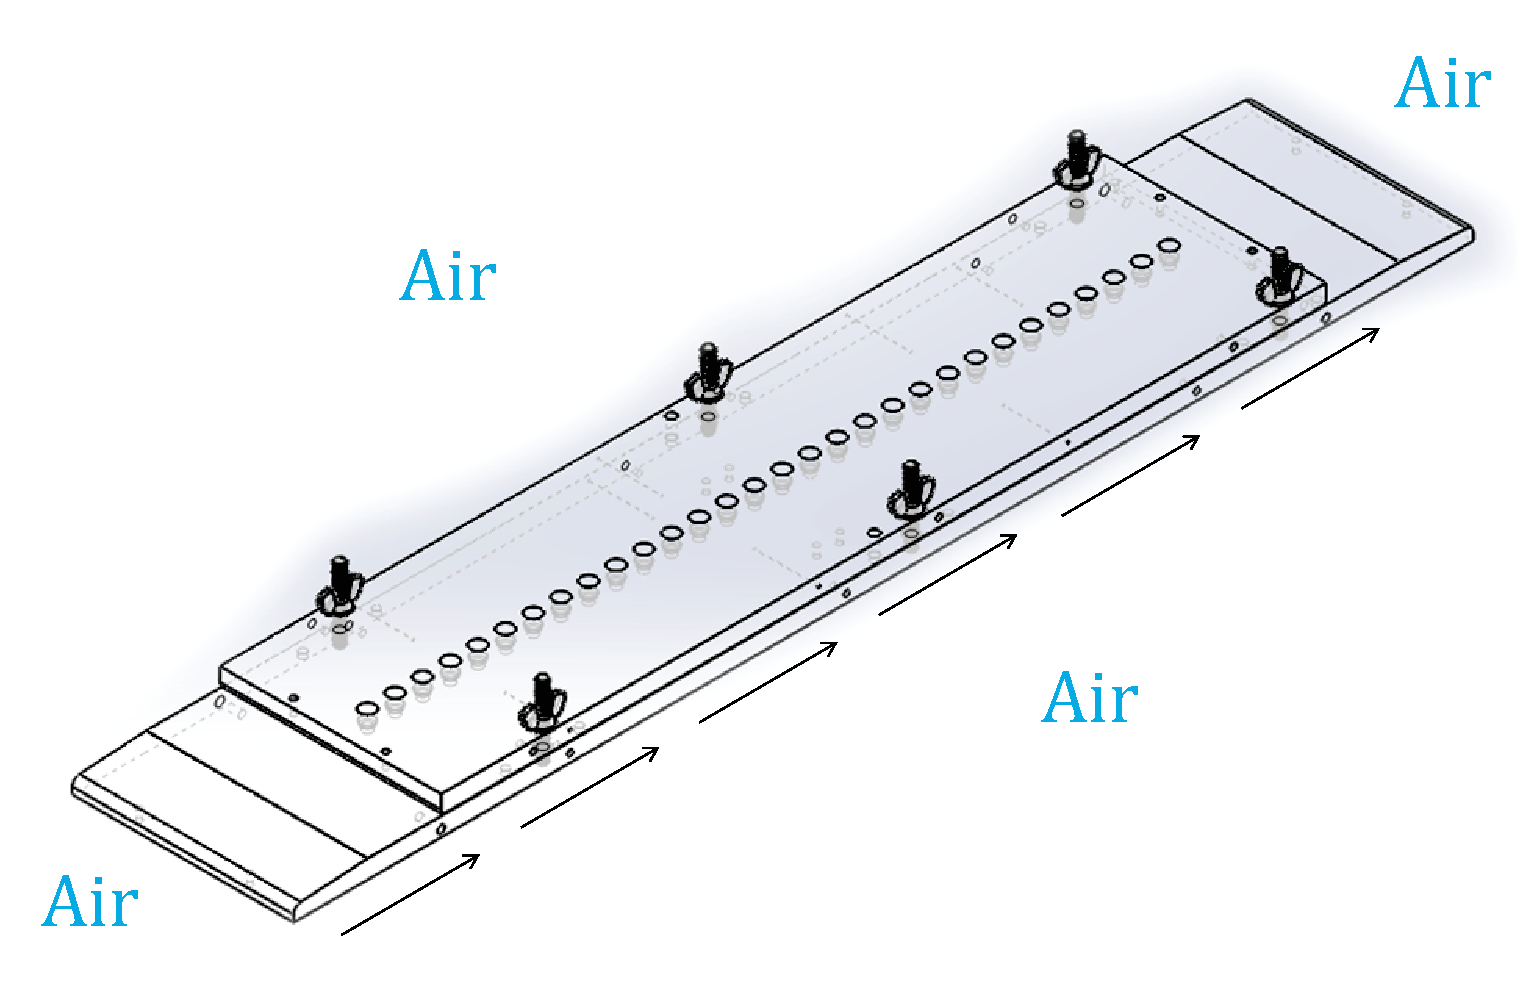
\includegraphics[scale=0.6]{ALD_machine.eps}
	\caption{CAD model of the atomic layer deposition machine. The holes at the top represent the inlets through which the chemical reactants will enter. The conveyor belt at the bottom moves the web in the direction of the arrows as the chemicals are deposited. The machine has open boundaries which may cause reactions with air, and lead to imperfections in the deposition.}
	\label{fig:ALD_machine}
\end{figure}
%
\begin{figure}
	\centering
	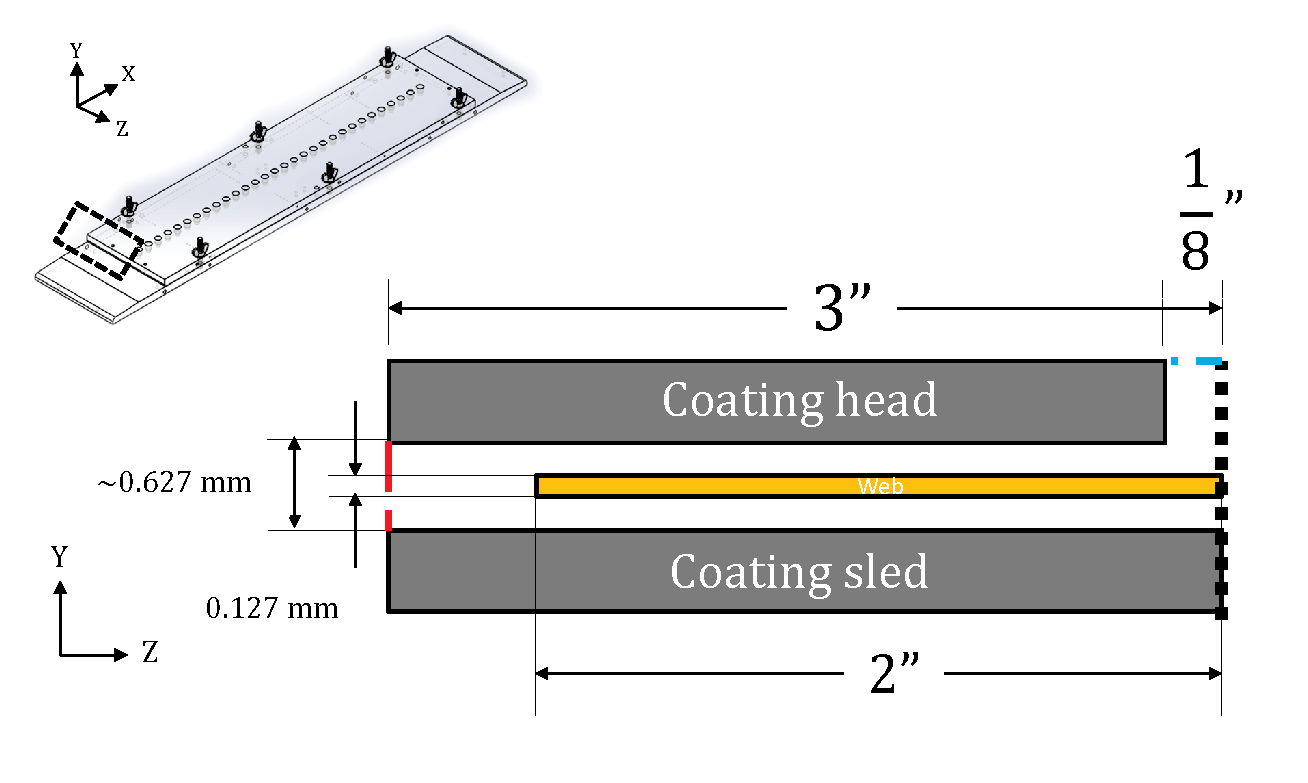
\includegraphics[scale=0.75]{ALD_zoom.eps}
	\caption{Cross-sectional view of the ALD machine. The black dotted line on the right represents a symmetry boundary condition. The coating head and sled are made of solid aluminum. The web on which the reactants are deposited is a polymer. The blue dotted line represents the gas inlets, and the red dotted line represents the open boundary conditions.}
	\label{fig:ALD_zoom}
\end{figure}
%
\begin{figure}
	\centering
	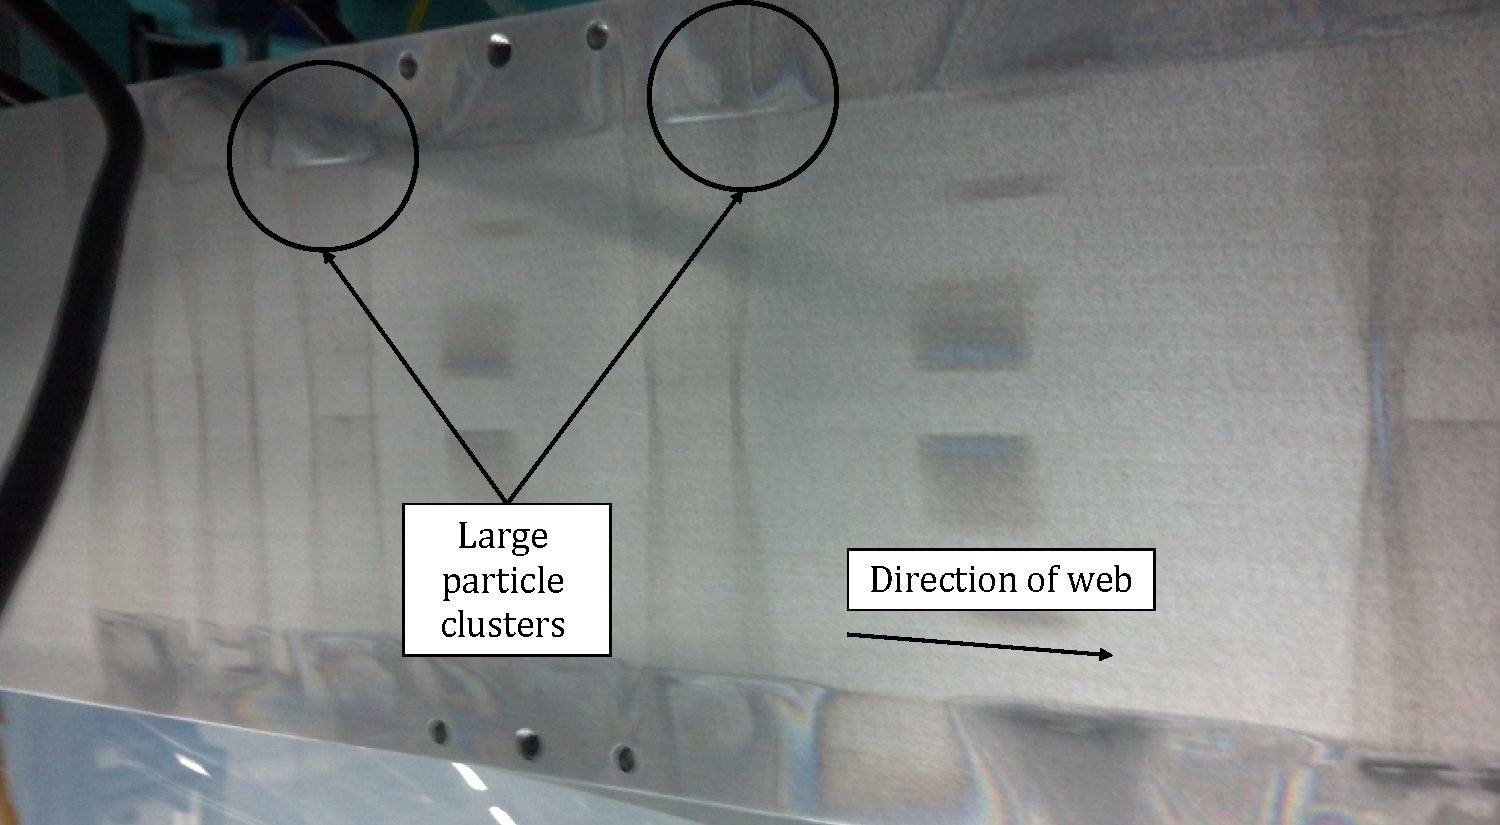
\includegraphics[scale=0.5]{reaction.eps}
	\caption{View of the coating sled after a deposition was performed. The picture shows that large particle clusters are formed at the open boundaries. Our hypothesis is that air reacts at the edges with the $\mathrm{TMA}$ reactant.}
	\label{fig:reaction}
\end{figure}

The goals of this study are to develop a profound understanding of the advective and diffusive transport phenomena which dominate the spatial and temporal distribution of reactants, and to create a novel computational environment for optimally designing the layout, the geometry and the operating parameters of the gas source head assembly.

%The first set of goals includes modeling the flow in and across the gas source head as well as the distribution of reactants across the substrate surface. In the case of porous substrate a major goal is to predict the penetration of reactants of the porous surface and the in-plane and through-thickness distributions. The latter is challenging as multiple length-scales need to be considered, ranging from the dimensions of the gas source head, the size of the gap between head and substrate, and the pore size of the substrate.

A computational fluid dynamics model was developed to predict the distribution of reactants. The model used an incompressible Navier-Stokes flow model which advects the concentration field of the reactants, augmented with a Brinkman model \citep{BP:03} for modeling the flow in porous media. This model was applied to a gas source head configuration which is used by ALD Nanosolutions and verified against experimental data. Various inlet configurations were studied. The Brinkman model was furthermore augmented to simulate a moving porous material rather than a static one. This model was applied to the moving porous substrate layer that transports the web on which the reactants are applied. 

We created the foundation for a level-set based geometry optimization framework where the flow is predicted by the extended finite element method (XFEM). Expanding on previous work we expanded our level-set/XFEM optimization capabilities to three-dimensional problems, an essential capability to design the layout of the gas source head. The level-set XFEM model was expanded to handle ``fluid-void'' and ``fluid-solid'' problems in three dimensions, which was essential to model the interaction of the reactants with the porous substrates.

The Brinkman flow modeling research helped to understand how the porous substrate captures and prevents the transport of the reactants. Our initial work on modeling the penetration of reactants into porous substrate was targeted at gaining insight into the effects of the different timescales involved in the transport phenomena. Our current work with the Brinkman model targets the penetration and transport of the reactants into the porous substrate when the web is in motion. Our work with the level-set XFEM optimization framework aimed at developing robust methods to model ``fluid-void'' and ``fluid-solid'' problems in three dimensions and optimize the porous substrate in order to minimize the areas of mixing zones.

% 
% \keywords{eXtended Finite Element Method \and Topology Optimization \and
% Solid Isotropic Material with Penalization \and Level Set Methods \and Additive Manufacturing \and 3D Printing}
% 
% \end{abstract}

% -----------------------------------------------------------------------------

\section{Conclusions}
\label{sec:ALD_conclusions}

With respect to the CFD modeling, we have developed a framework to model fluid-structure interaction using a Brinkman model in which the structure has the capability to displace. This will play a key role in the verification of the experimental data obtained from ALD NanoSolutions. At the same time, our level-set XFEM framework allows us to model complex ``fluid-fluid'' and ``fluid-solid'' problems and optimize the area where the reactants mix, reducing imperfections in the atomic deposition and allowing for fast new design iterations.

We plan to expand our scalar transport model to simulate multiple scalar transport fields and research the interaction of the reactant with the outside sources, such as air.

We further plan to expand and apply our level-set/XFEM optimization framework to design the geometry of gas source heads.

% -----------------------------------------------------------------------------
% Acknowledgement

% \subsection*{Acknowledgement}
% 
% The authors acknowledge the support of the National Science Foundation under grant EFRI-ODISSEI  1240374 and CBET 1246854. The opinions and conclusions presented in this paper are those of the authors and do not necessarily reflect the views of the sponsoring organization.

% -----------------------------------------------------------------------------
% Bibliography

% \bibliographystyle{etc/spbasic}
% \bibliography{etc/JabRefDatabase}

% \end{document}
